\documentclass[tikz,border=0pt]{standalone}
\usepackage[american]{circuitikz}
\usetikzlibrary{arrows.meta,calc,positioning,decorations.pathmorphing,patterns}
\definecolor{zyloTeal}{HTML}{174A5B}
\definecolor{zyloTealTwo}{HTML}{246B7A}
\definecolor{zyloInk}{HTML}{1F2933}
\definecolor{zyloSoft}{HTML}{EAF4F4}
\definecolor{zyloPaper}{HTML}{F8FAFB}
\definecolor{zyloLine}{HTML}{44606B}
\definecolor{zyloOrange}{HTML}{D97706}
\begin{document}
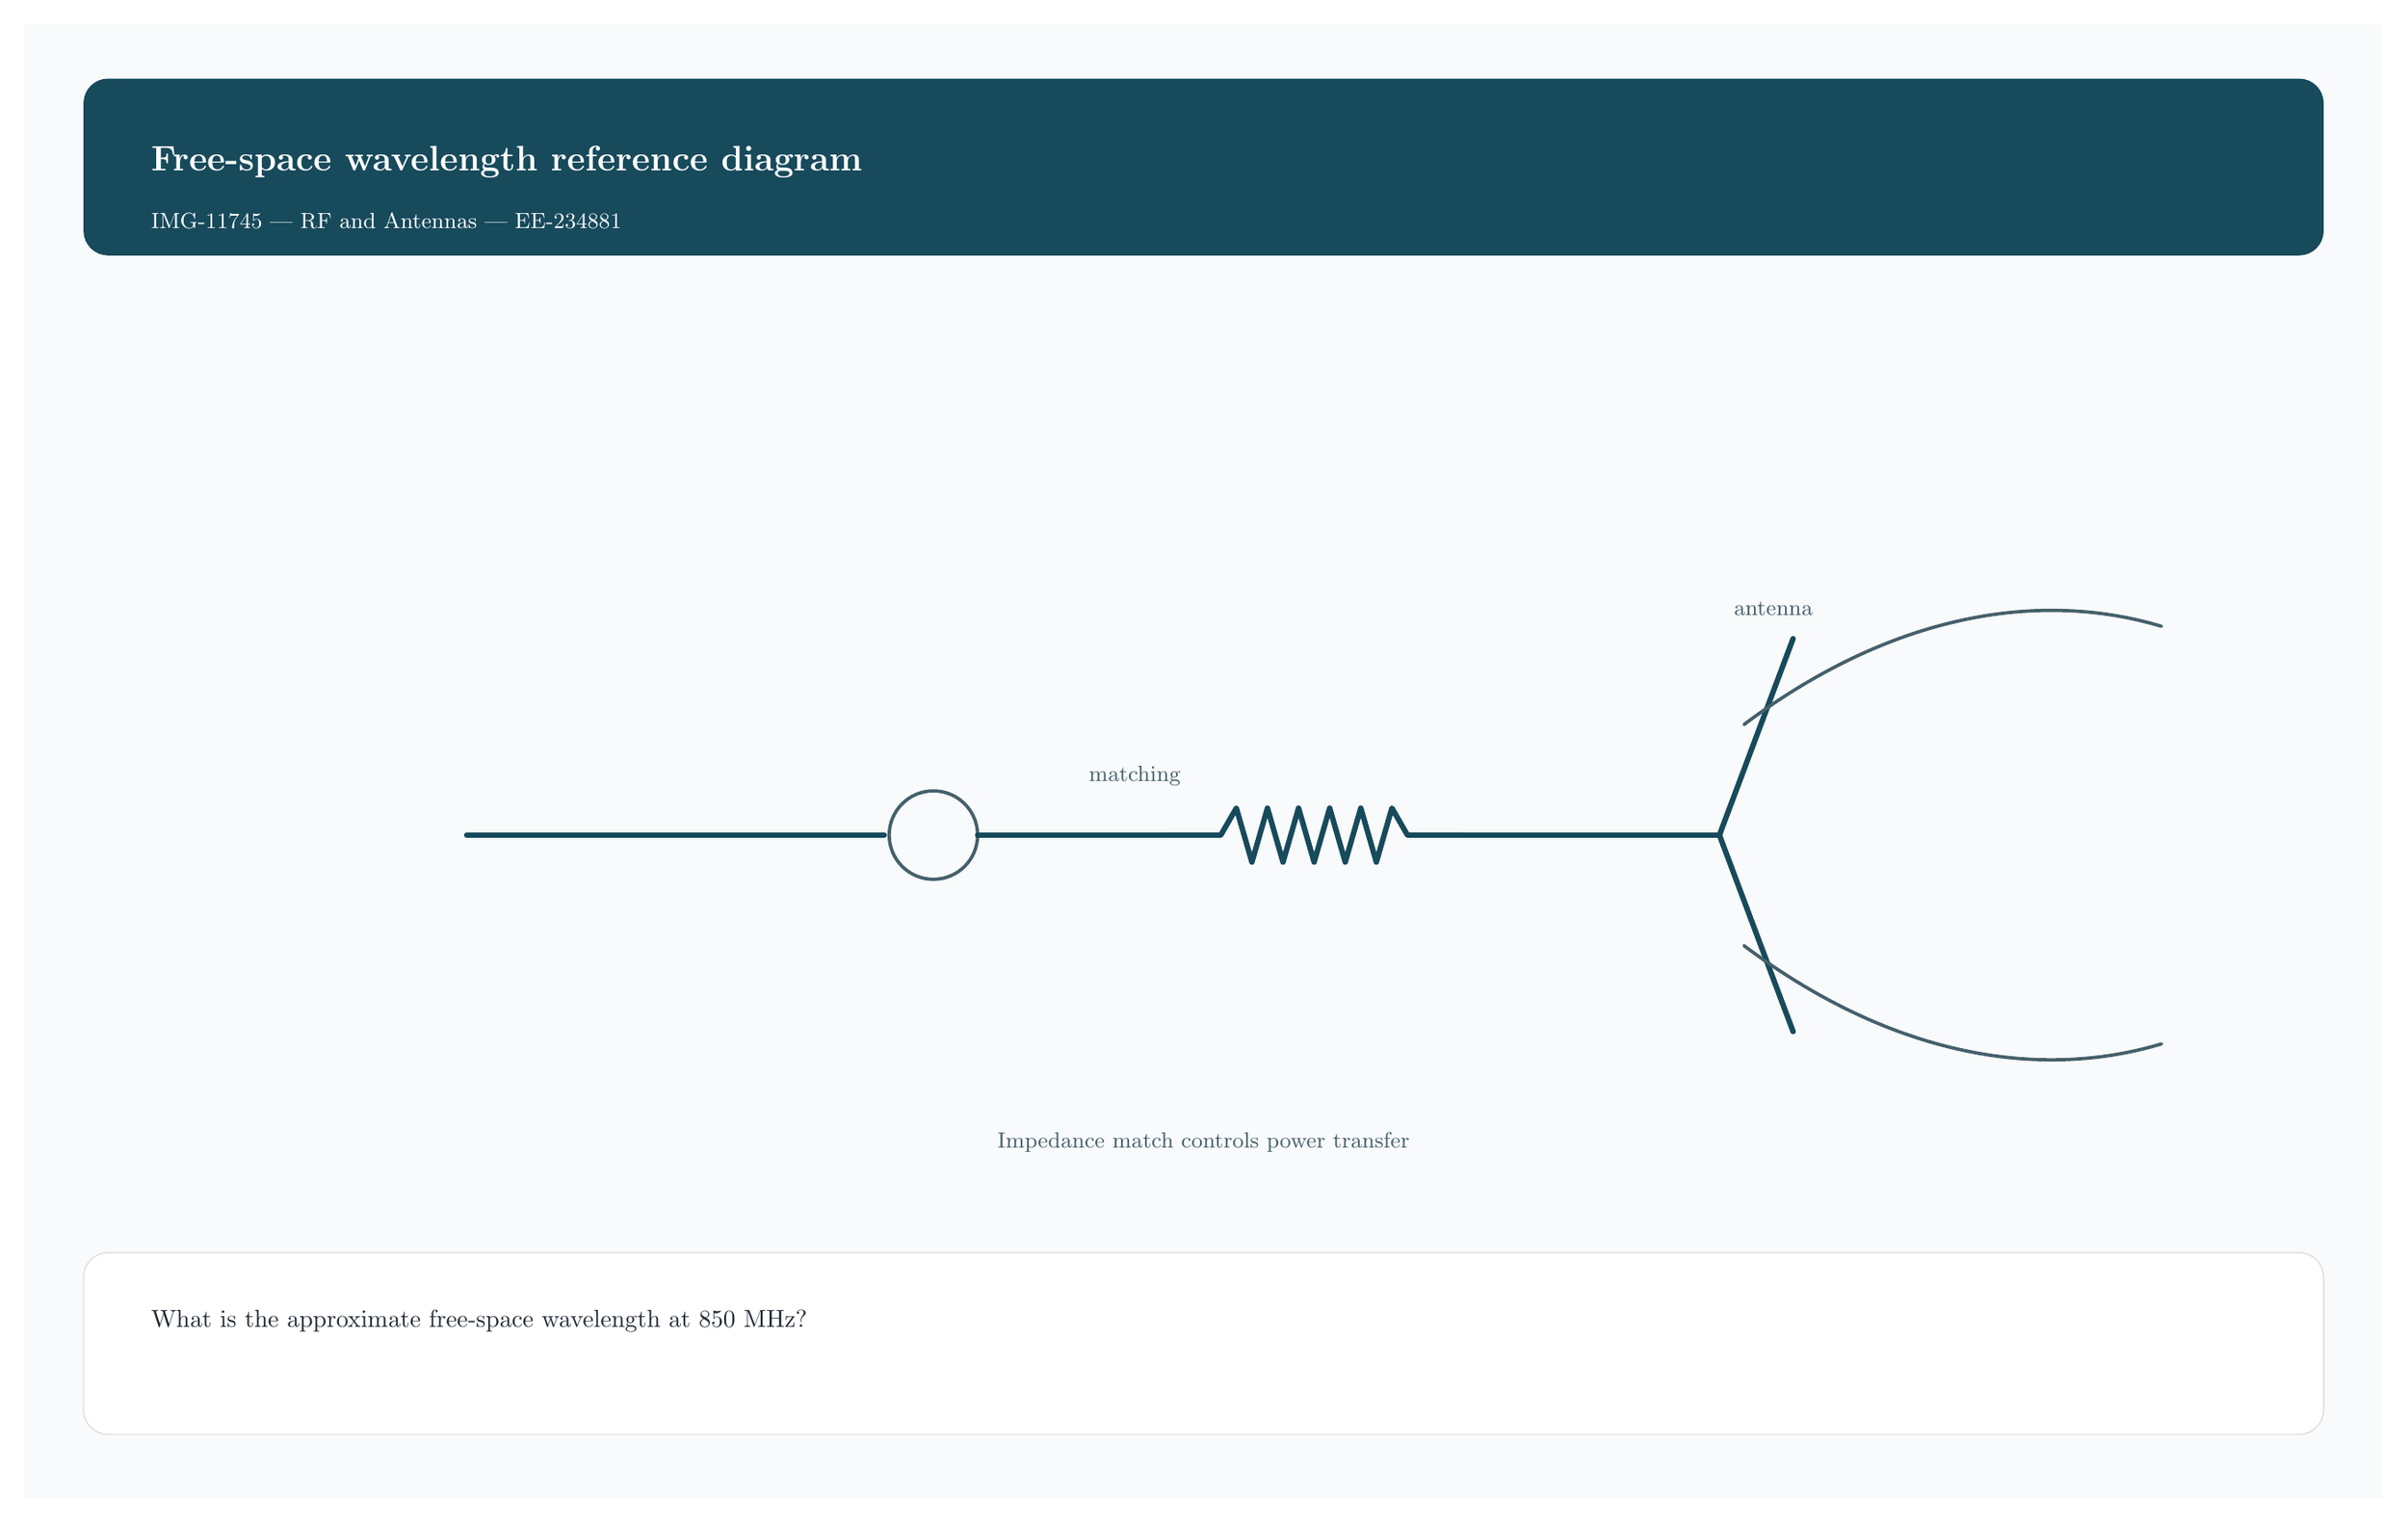
\begin{tikzpicture}[x=1pt,y=-1pt,>=Latex,line cap=round,line join=round]
\path[fill=zyloPaper] (0,0) rectangle (960,600);
\path[fill=zyloTeal,rounded corners=10pt] (24,22) rectangle (936,94);
\node[anchor=west,text=white,font=\bfseries\Large] at (48,56) {Free-space wavelength reference diagram};
\node[anchor=west,text=white!82,font=\small] at (48,80) {IMG-11745 | RF and Antennas | EE-234881};
\tikzset{wire/.style={draw=zyloTeal,line width=2.2pt},thinwire/.style={draw=zyloLine,line width=1.35pt},accent/.style={draw=zyloOrange,line width=2.2pt},box/.style={draw=zyloTealTwo,fill=zyloSoft,line width=1.5pt,rounded corners=8pt}}
\draw[wire] (180,330) -- (350,330);
\draw[thinwire] (370,330) circle (18);
\draw[wire] (388,330) -- (465,330);
\draw[wire] (465,330) -- (487,330) -- (487,330) -- (493.333,319) -- (499.667,341) -- (506,319) -- (512.333,341) -- (518.667,319) -- (525,341) -- (531.333,319) -- (537.667,341) -- (544,319) -- (550.333,341) -- (556.667,319) -- (563,330) -- (585,330);
\draw[wire] (585,330) -- (690,330);
\draw[wire] (690,330) -- (720,250); \draw[wire] (690,330) -- (720,410);
\draw[thinwire] (700,285) .. controls (760,240) and (820,230) .. (870,245); \draw[thinwire] (700,375) .. controls (760,420) and (820,430) .. (870,415);
\node[font=\small,text=zyloLine] at (452,306) {matching}; \node[font=\small,text=zyloLine] at (712,238) {antenna};
\node[font=\small,text=zyloLine] at (480,455) {Impedance match controls power transfer};
\path[draw=black!15,fill=white,rounded corners=10pt] (24,500) rectangle (936,574);
\node[anchor=west,text width=860pt,align=left,text=zyloInk,font=\normalsize] at (48,528) {What is the approximate free-space wavelength at 850 MHz?};
\end{tikzpicture}
\end{document}
